\section{Results and Discussion}
\label{sec:results}

Across the 495 planned trials, 430 yielded successfully verified solutions, 20 encountered timeouts, and 45 were blocked by expected MIP license limitations. No solver generated an invalid placement.

\subsection{Structural Comparison of SAT Encodings}
As instance size grows, the structural disparities of CNF generation become stark. At $N=100$, all encodings instantiate identical 10,000 primary binary variables but vary widely in auxiliary metrics. The Pairwise encoding requires zero auxiliary variables but scales poorly, producing 1,646,900 clauses. The Sequential Counter encoding generates the second-fewest clauses (117,812) at the cost of the highest auxiliary count (39,402). The Product encoding achieves the most compact configuration, producing 116,672 clauses and 9,492 auxiliary variables. Binary and Commander encodings balance these metrics. 

\begin{figure}[htbp]
\centering
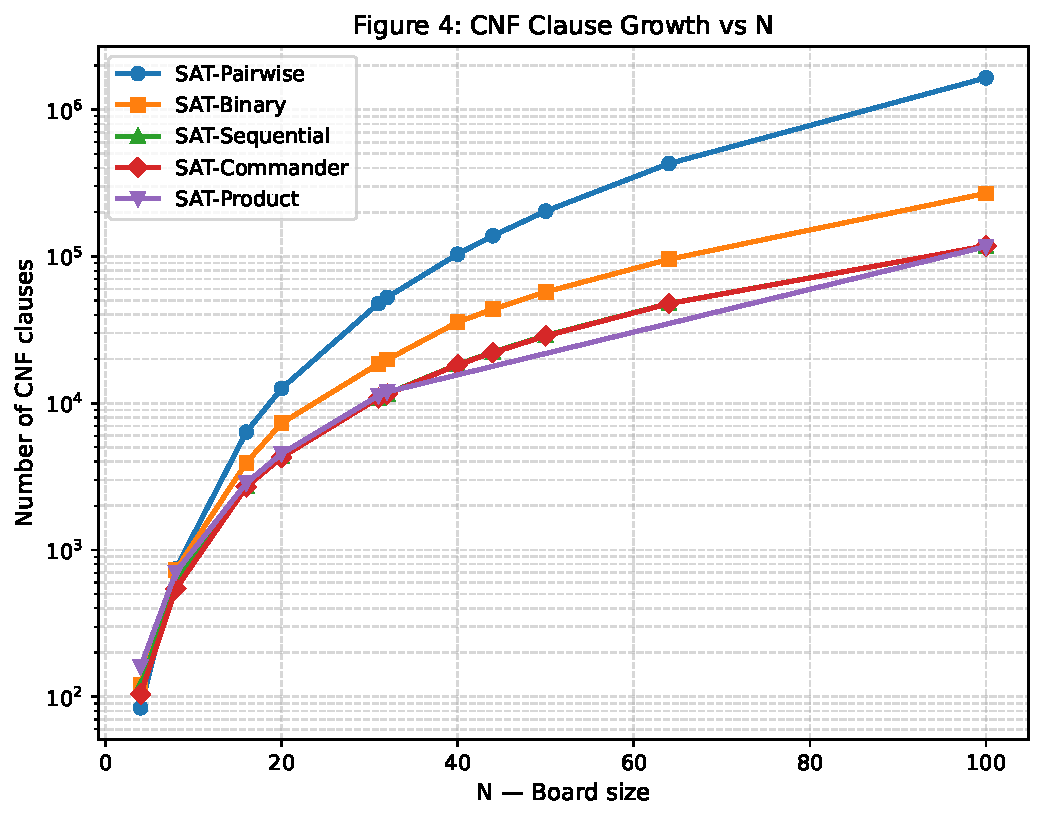
\includegraphics[width=0.8\textwidth]{../../results/figures/full/fig04_sat_clause_growth.pdf}
\caption{SAT CNF Clause Growth}
\label{fig:sat_clause_growth}
\end{figure}

\begin{figure}[htbp]
\centering
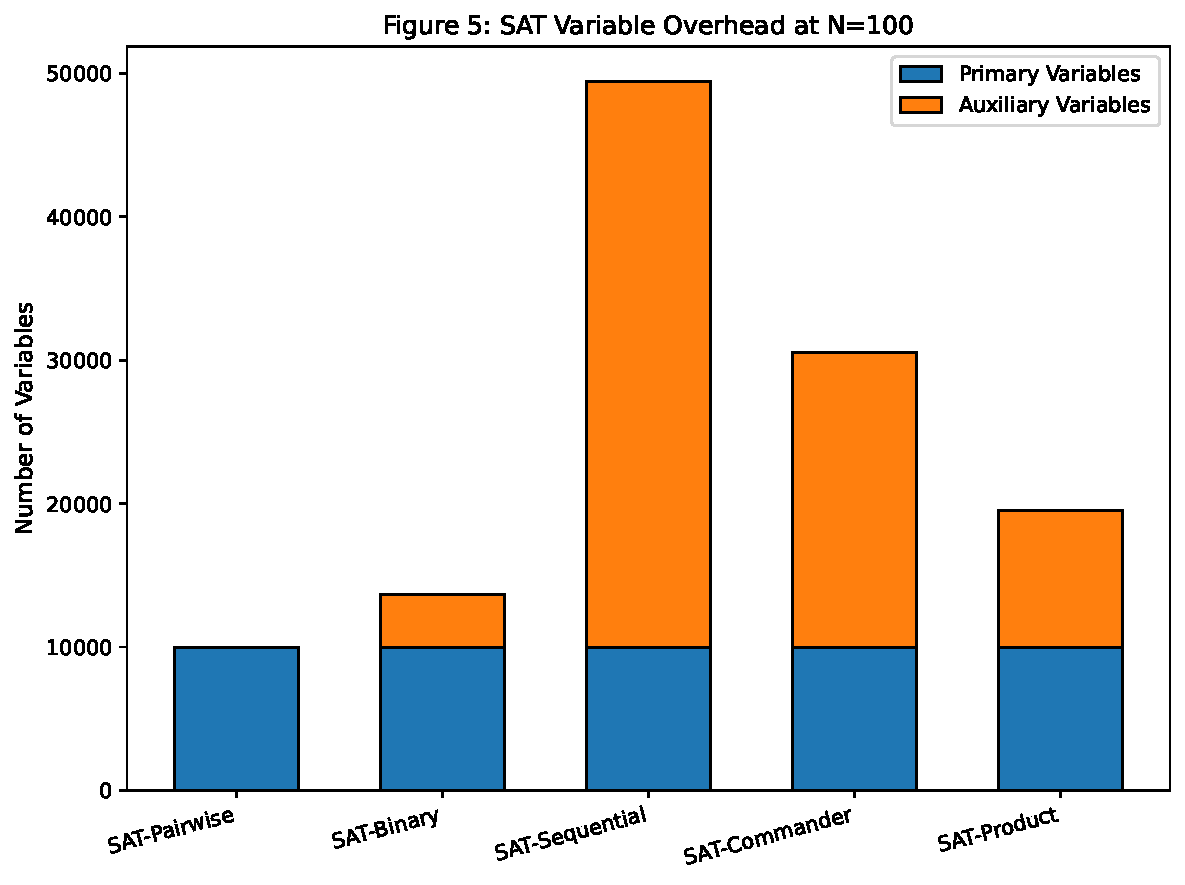
\includegraphics[width=0.8\textwidth]{../../results/figures/full/fig05_sat_variable_overhead_n100.pdf}
\caption{SAT Auxiliary Variable Overhead}
\label{fig:sat_aux_overhead}
\end{figure}

\subsection{Runtime Performance of SAT Encodings}
The resolution time for SAT formulations proves that clause count is an inadequate predictor of performance. 

\begin{figure}[htbp]
\centering
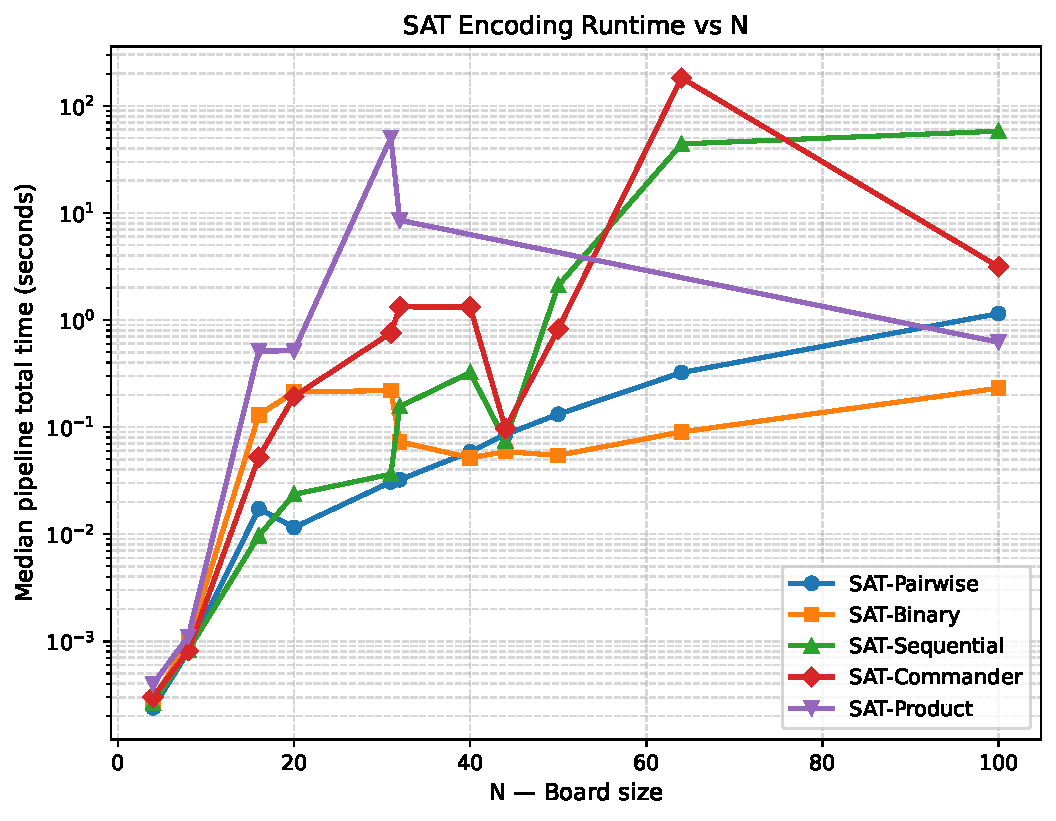
\includegraphics[width=0.8\textwidth]{../../results/figures/full/fig01_sat_runtime_vs_n.pdf}
\caption{SAT Runtime vs N}
\label{fig:sat_runtime}
\end{figure}

At $N=100$, the SAT-Binary encoding achieved the fastest median pipeline runtime of 0.231 seconds. In stark contrast, the SAT-Sequential encoding, despite producing minimal clauses, recorded the slowest median runtime of 58.077 seconds. The clause-heavy SAT-Pairwise encoding successfully completed the search in a median time of 1.148 seconds. 

\subsection{Non-monotonic Search Behavior of Product Encoding}
While SAT-Product reliably solved small sizes and successfully resolved $N=100$ (median 0.620s), it completely failed at intermediate sizes ($N \in \{40, 44, 50, 64\}$), resulting in a timeout for all 5 repetitions.

\begin{figure}[htbp]
\centering
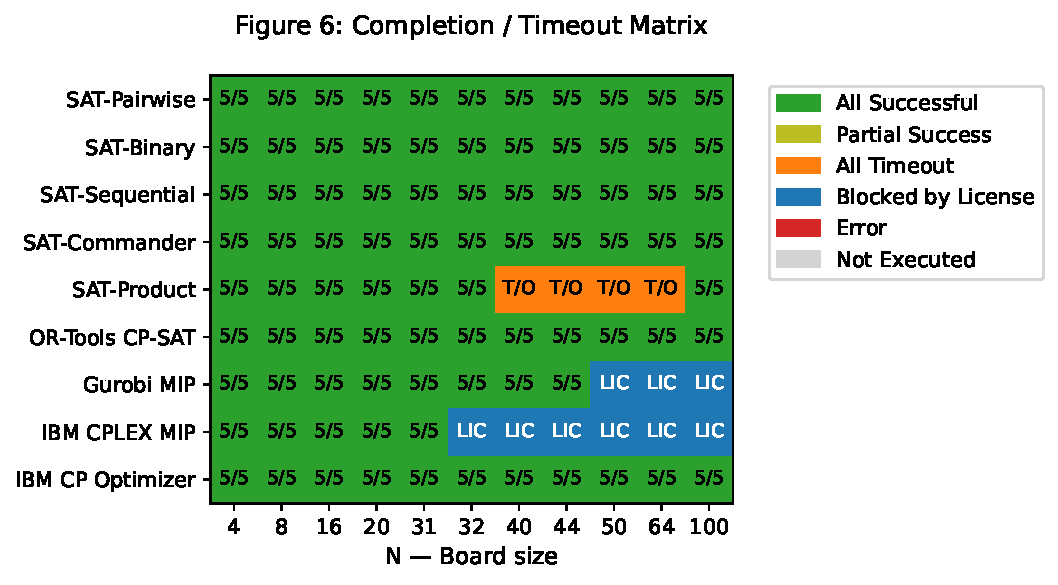
\includegraphics[width=0.8\textwidth]{../../results/figures/full/fig06_completion_matrix.pdf}
\caption{Completion Matrix}
\label{fig:completion_matrix}
\end{figure}

This non-monotonic scaling underscores the sensitivity of CDCL solvers to heuristic traps. Under Glucose3's \texttt{solver\_default} policy, the specific auxiliary-variable structure of Product at intermediate bounds may force the search into pathological branching spaces. However, these are potential contributing factors; analyzing the exact causes of this behavior requires further experimental study of internal solver traces and variable ordering.

\subsection{Performance of Exact Solvers}
Native Constraint Programming (CP) architectures demonstrated highly favorable scaling characteristics. 

\begin{figure}[htbp]
\centering
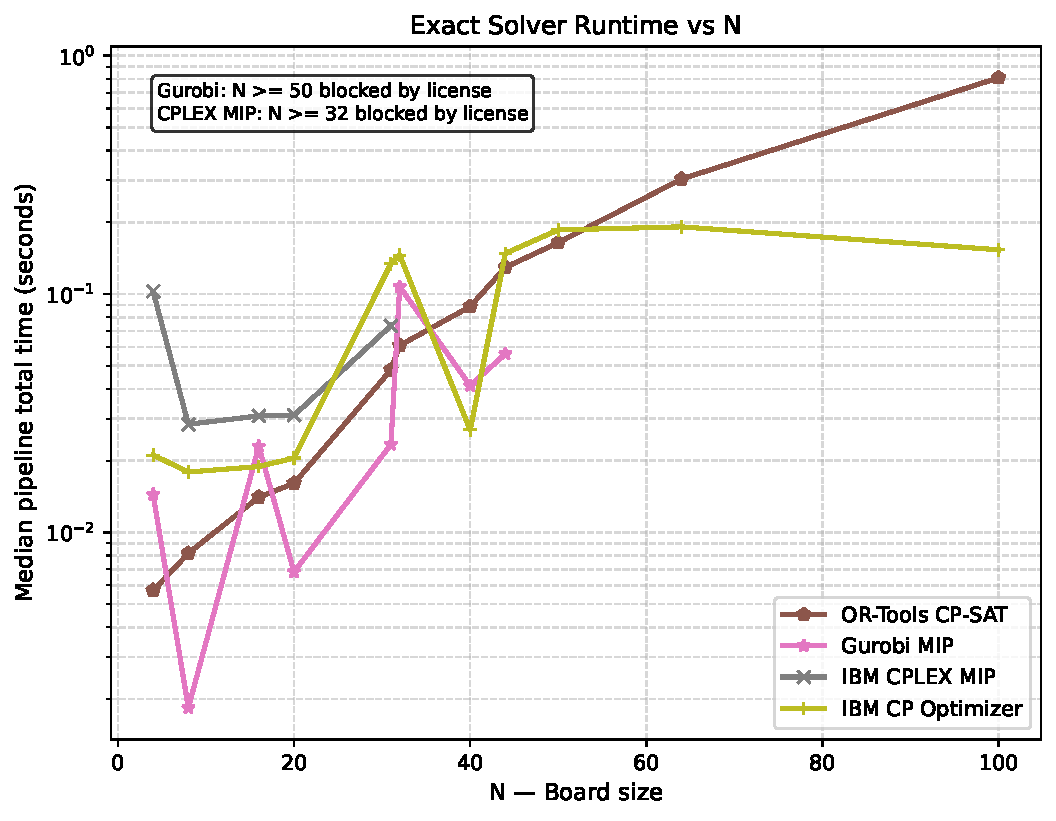
\includegraphics[width=0.8\textwidth]{../../results/figures/full/fig02_exact_solver_runtime_vs_n.pdf}
\caption{Exact Solver Runtime vs N}
\label{fig:exact_runtime}
\end{figure}

Both IBM CP Optimizer and OR-Tools CP-SAT maintained 100\% reliability up to $N=100$. The CP Optimizer solver established itself as remarkably efficient.
The MIP solvers successfully solved bounds within their Community Edition license constraints.

\subsection{Cross-Paradigm Comparison at N=100}
At $N=100$, seven methods successfully executed. The IBM CP Optimizer achieved the lowest median runtime of 0.153 seconds.

\begin{figure}[htbp]
\centering
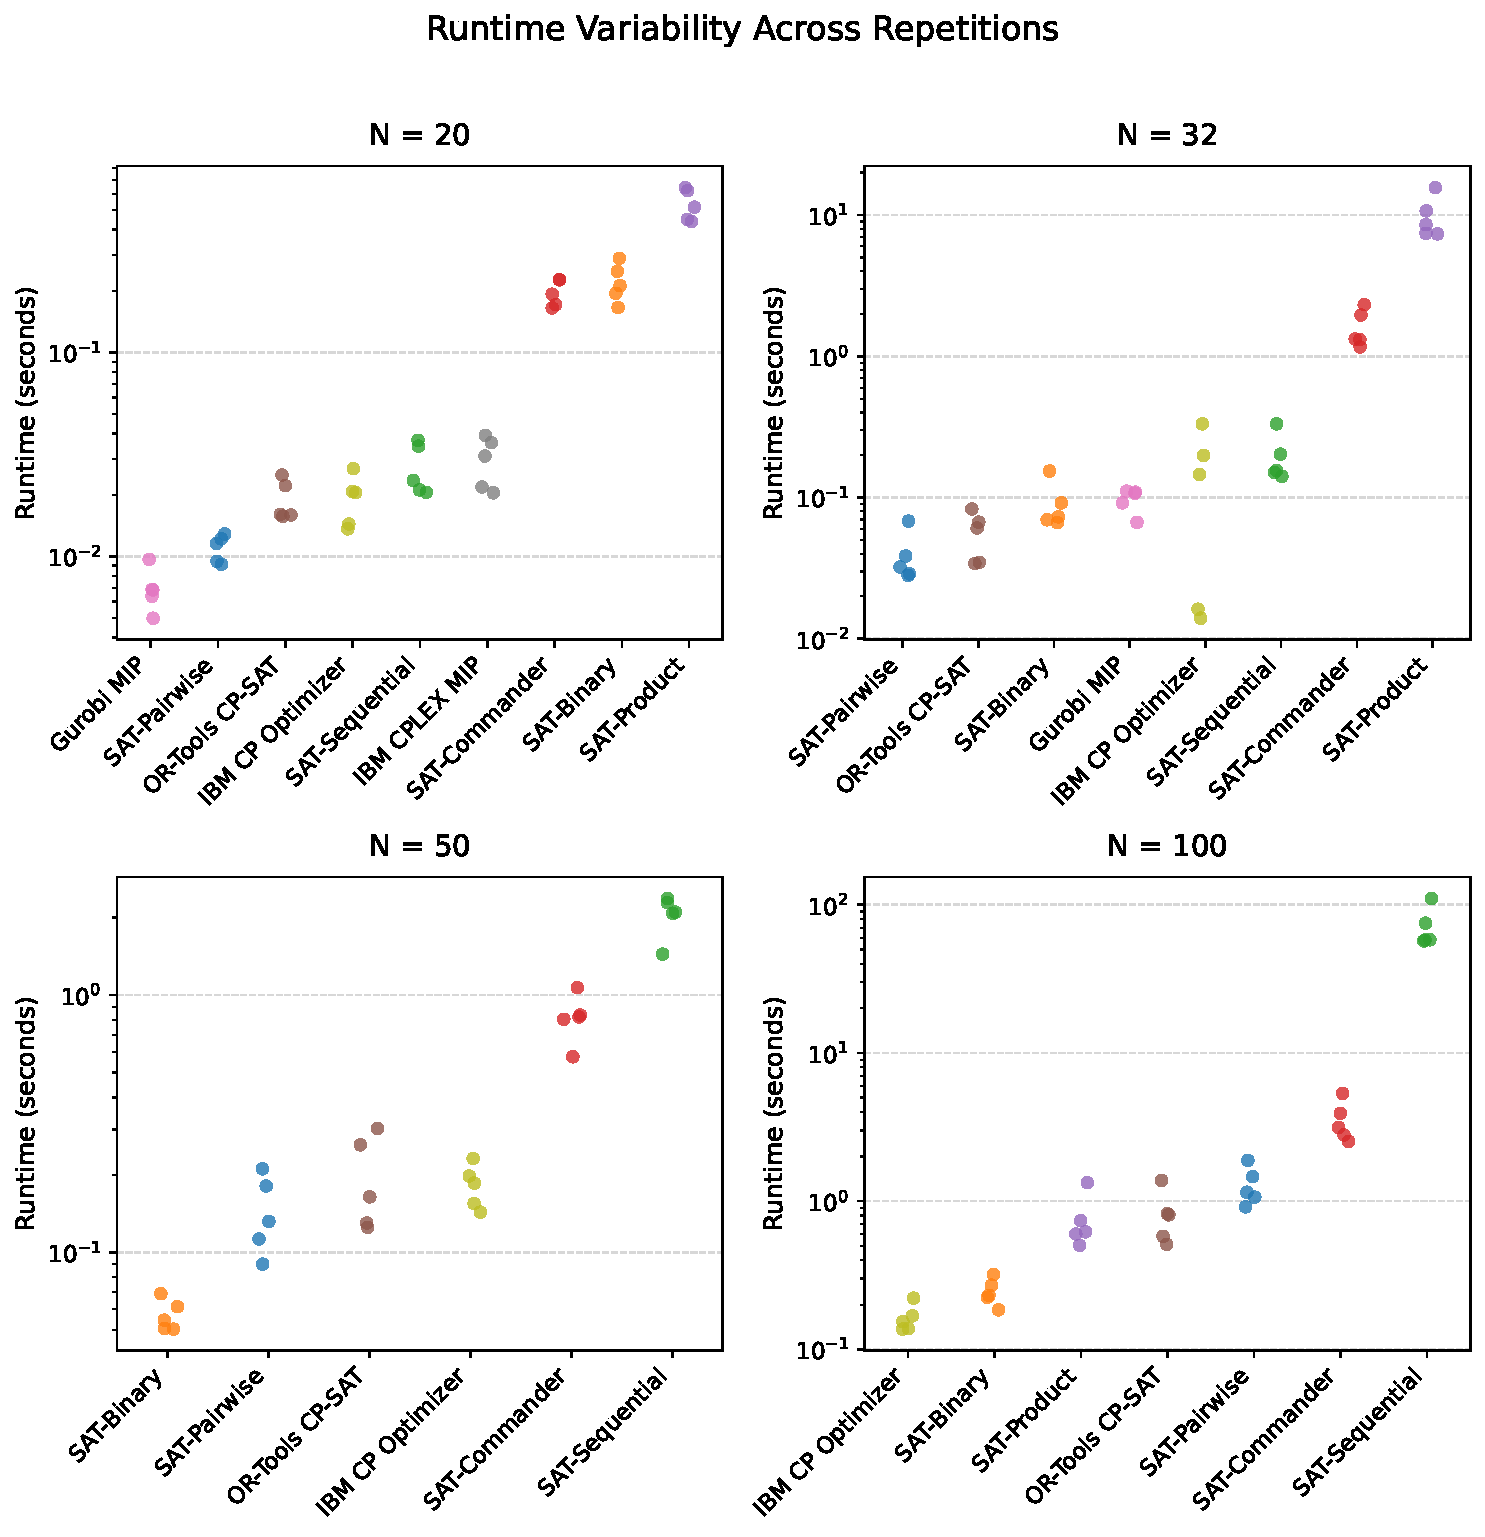
\includegraphics[width=0.8\textwidth]{../../results/figures/full/fig07_runtime_variability.pdf}
\caption{Runtime Variability}
\label{fig:runtime_variability}
\end{figure}

Remarkably, the booleanized SAT-Binary formulation tracked incredibly close at 0.231 seconds, outpacing OR-Tools CP-SAT (0.808 seconds). 

\begin{table}[h]
\centering
\caption{SAT Encoding Structural Complexity at N=100}
\begin{tabular}{@{}lrrr@{}}
\toprule
Encoding & Primary Variables & Auxiliary Variables & Clauses \\
\midrule
Pairwise & 10,000 & 0 & 1,646,900 \\
Binary & 10,000 & 3,678 & 269,024 \\
Sequential & 10,000 & 39,402 & 117,812 \\
Commander & 10,000 & 20,536 & 118,092 \\
Product & 10,000 & 9,492 & 116,672 \\
\bottomrule
\end{tabular}
\label{tab:sat_structure}
\end{table}

\begin{table}[h]
\centering
\caption{Cross-Paradigm Comparison at N=20}
\begin{tabular}{@{}lrr@{}}
\toprule
Method & Success Rate & Median Runtime (s) \\
\midrule
Gurobi MIP & 5/5 & 0.0068 \\
SAT-Pairwise & 5/5 & 0.0115 \\
OR-Tools CP-SAT & 5/5 & 0.0160 \\
IBM CP Optimizer & 5/5 & 0.0205 \\
SAT-Sequential & 5/5 & 0.0235 \\
IBM CPLEX MIP & 5/5 & 0.0309 \\
SAT-Commander & 5/5 & 0.1928 \\
SAT-Binary & 5/5 & 0.2124 \\
SAT-Product & 5/5 & 0.5150 \\
\bottomrule
\end{tabular}
\label{tab:n20}
\end{table}

\begin{table}[h]
\centering
\caption{Cross-Paradigm Comparison at N=100}
\begin{tabular}{@{}lrr@{}}
\toprule
Method & Success Rate & Median Runtime (s) \\
\midrule
IBM CP Optimizer & 5/5 & 0.153 \\
SAT-Binary & 5/5 & 0.231 \\
SAT-Product & 5/5 & 0.620 \\
OR-Tools CP-SAT & 5/5 & 0.808 \\
SAT-Pairwise & 5/5 & 1.148 \\
SAT-Commander & 5/5 & 3.143 \\
SAT-Sequential & 5/5 & 58.077 \\
Gurobi MIP & N/A & BLOCKED\_LICENSE \\
IBM CPLEX MIP & N/A & BLOCKED\_LICENSE \\
\bottomrule
\end{tabular}
\label{tab:n100}
\end{table}

\begin{figure}[htbp]
\centering
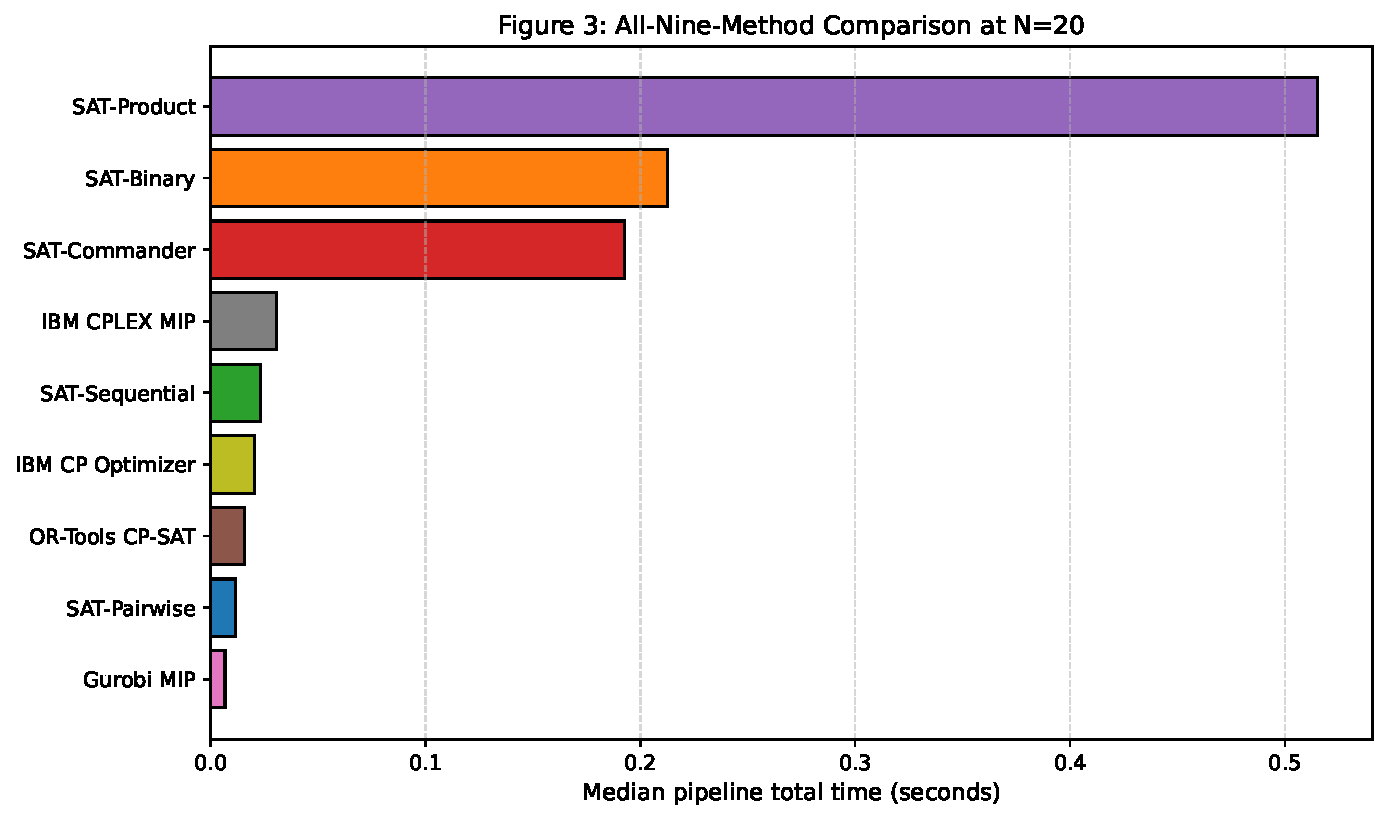
\includegraphics[width=0.8\textwidth]{../../results/figures/full/fig03_all_methods_n20.pdf}
\caption{All Nine Methods at N=20}
\label{fig:all_methods_n20}
\end{figure}

\begin{table}[h]
\centering
\caption{Completion Reliability Across All 495 Trials}
\begin{tabular}{@{}lrrr@{}}
\toprule
Method & Successful Runs & Timeout Runs & License Blocked Runs \\
\midrule
SAT-Pairwise & 55 & 0 & 0 \\
SAT-Binary & 55 & 0 & 0 \\
SAT-Sequential & 55 & 0 & 0 \\
SAT-Commander & 55 & 0 & 0 \\
SAT-Product & 35 & 20 & 0 \\
OR-Tools CP-SAT & 55 & 0 & 0 \\
IBM CP Optimizer & 55 & 0 & 0 \\
Gurobi MIP & 40 & 0 & 15 \\
IBM CPLEX MIP & 25 & 0 & 30 \\
\midrule
\textbf{Total} & \textbf{430} & \textbf{20} & \textbf{45} \\
\bottomrule
\end{tabular}
\label{tab:reliability}
\end{table}
